\documentclass[11pt,a4paper]{ltjsarticle}
% ltjsarticle: lualatex 用の 日本語 documentclass
% 他のタイプセットエンジンを使ってビルドする場合は、 \documentclass[dvipdfmx]{jsarticle} などとする。
%https://takataninote.com/tex/contents.html
%https://guides.lib.kyushu-u.ac.jp/LaTeX-LectureNote/basic

\usepackage{luatexja}

\usepackage{graphicx}

\usepackage{hyperref}
\usepackage{amsmath}
\usepackage{amssymb}
\usepackage{mathtools}
\usepackage{xcolor}

\setcounter{tocdepth}{3}

\title{The theory of EIT in Nitrogen Vacancy }
\author{工学院電気電子系25M12095 阿部 李星}
\begin{document}

\maketitle

% 目次の出力
\tableofcontents


\clearpage




% ここからが本文


\section{背景}
EIT(Electromagnetically Induced Transparency)とは、2つのレーザーを用いることで生じる量子干渉効果により、特定の周波数周辺において吸収率が減少する現象である。
EITは、アルカリ原子の気体中などで観測されていたため、EITを実現する材質は気体に限られていると考えられてきた。しかし、近年の実験機器
や測定技術の進歩により、固体中においてもEITが観測されるようになった。一般に、固体状の材質は既存のデバイスとの融合が容易のため、EITを動作原理と
とする技術が提案されてきた。ところが、固体中のEITの観測は低温に限定されていたため、実用化に向けて温度向上が求められている。

 本稿では、3準位系におけるEITの実現条件を述べ、その実現条件がどのパラメータに依存しているかを見ていく。
そして、3準位系での理論を4準位系に拡張し、NVセンターにおけるEITの実現条件を議論する。


\section{前提知識}

\subsection{電気双極子相互作用ハミルトニアンと回転波変換}

\subsection{Kramers - Kroning の分散関係式}

\subsection{Master方程式}


\subsection{Ac Stark ShiftとEITの違い}
先述のとおり、EITはある周波数領域で吸収率が低下する現象であると述べたが、
同様の現象を示す効果が存在する。それが、AC Stark Shift(Autler-towness Shift, ATS)である。
AC Stark Shift とは、Stark Shiftの一種であるが、ATSは交流電場、つまり光を入射させたときの
Stark Shiftを指す。
下記に両者の効果を図として示す。(a)がEITであり、(b)がATS である。
実験結果を見ると、吸収率が減少する領域の広さに違いがあるのみで、両者の区別は難しい。
しかし、これらの効果が引き起こされる原因は異なる。

\section{3準位系でのEIT}




\begin{figure}[htbp]
  \begin{center}
  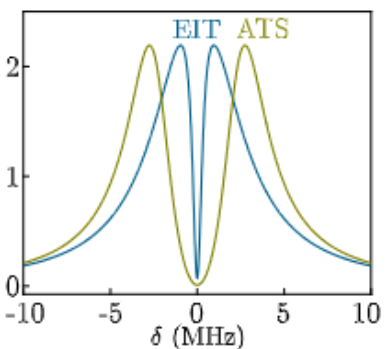
\includegraphics[width=50mm]{image/EIT_and_ATS.png}
  \caption{EITとATSの比較}
  \end{center}
\end{figure}



まず、EITは、どの励起準位とも遷移関係をもたない暗状態(Dark State)の存在によって、
吸収率が下がる。この効果は、2準位系ではみられず、一般に3準位系でみられるものである。
一方、ATSの場合、振動電場によって原子のスペクトルが変化することが
原因で生じる。吸収率のピーク間がEITよりもやや広いため、吸収率の谷が形成され、透過性を示す。
この効果は2準位系、3準位系でも実現が可能である。


{\color{red}※EITとAutler-towness効果の違いはDark stateの有無か？}



\subsection{3準位系におけるEITはどのようにして導出されるか}
EIT信号を導出する方法は、密度行列に基づく方法と、Dressed stateに基づく方法の2通りが
存在する。ここでは、密度行列に基づく方法で、EIT信号の導出を試みる。

何度も述べる通り、EITは主に、3準系で見られる現象だが、特に$\Lambda$ 系の文脈で語られることが多い。
そのため、以下では$\Lambda$系を単に3準位系と呼ぶことにする。

それでは、3準位系におけるEIT信号がどのようにして導出されるかを見ていく。まず、3準位系の各準位を下記の図のように定義する。
$| 1 \rangle,| 12\rangle$ が基底準位、$| 3 \rangle$ が励起準位であり、それぞれのエネルギー差は、
$\omega_{31},\omega_{32}$ と定義する。なお、準位間の遷移は2つのレーザー(Contorol,Probe)によって駆動される。


\begin{figure}[htbp]
  \begin{center}
  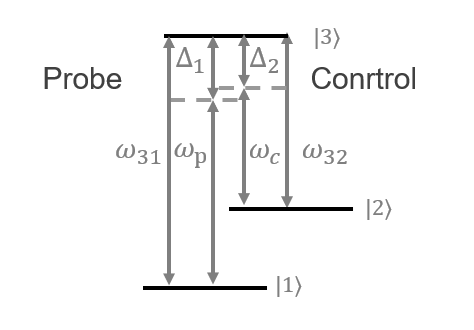
\includegraphics[width=50mm]{image/Lambda_system.png}
  \caption{EITとATSの比較}
  \end{center}
\end{figure}


\subsubsection{3準位系に相当するMaster方程式}
次に、3準位系における各パラメータについて述べる。まず、3準位系には、coherentなパラメータとしてRabi周波数($\Omega_{c},\Omega_{p}$) が
が存在する。$\Omega_c$ はControlのRabi周波数、$\Omega_p$ はProbeのRabi周波数である.一方、decoherentなパラメータとして自然放射レート(Spontaneous emission rate)、位相緩和レート(Dephasing rate)が存在する。
$| 3 \rangle$ から $| 1 \rangle$,$| 3 \rangle$ から $| 2 \rangle$ への自然放射レートをそれぞれ $\Gamma_{31},\Gamma_{32}$ として定義する。
そして、$| 1 \rangle$ を基準にした $| 2 \rangle,| 3 \rangle$ の位相緩和レートをそれぞれ $\gamma_{2 deph}, \gamma_{3 deph}$ と定義する。


{\color{red}※各パラメータは表にまとめたほうがみやすい}

以上のパラメータに基づき、3準位系の機構を記述する状態について述べる。

まず、レーザーとの相互作用を記述するハミルトニアンは次のように与えられる。



\begin{equation*}
 H_{ \mathrm{int} } = \frac{i}{\hbar} \left[ \Omega_{ \mathrm{p} } \left( t \right) | 3 \rangle \langle 1 | \mathrm{e}^{\mathrm{i} \omega_{\mathrm{p} } t}
         + \Omega_{\mathrm{c}} \left( t \right) | 3 \rangle \langle 2 | /mathrm{e}^{\mathrm{i}  \omega_{\mathrm{c} t}  } 
         + \mathrm{H.c.}      \right]
\end{equation*}

ただし、H.c. は、Hermitian conjugateの略であり、エルミート共役を意味する。

次に、この相互作用ハミルトニアン $H_{ \mathrm{int} }$ を回転波近似(Rotating wave approximation: RWA) に基づき、以下のように変形する。

\begin{equation*}
 H_{ \mathrm{int} } = \frac{i}{\hbar} \left[ \Omega_{\mathrm{p}} \left( t \right) | 3 \rangle \langle 1 | \mathrm{e}^{\mathrm{i} \Delta_{1} t}
         + \Omega_{\mathrm{c}} \left( t \right) | 3 \rangle \langle 2 | /mathrm{e}^{\mathrm{i} \Delta_{2} t}   
         + \mathrm{H.c.}      \right]
\end{equation*}


ここで、$\Delta_{1} = \omega_{31} - \omega_{p}$ はProbeのSingle photon detuning、
$\Delta_{2} = \omega_{32} - \omega_{c}$ はControlのSingle photon detuninと呼ぶ。


一般に、自然放射などの外界との相互作用を含む状態の時間発展は、Schrodinger 方程式では記述しきれない。
外界との相互作用を含む系(混合系)の状態は、一つの量子状態のみで記述できず、その量子状態が古典的な確率で混ぜ合わさった状態(混合状態)
とし、この$\rho(t)$ の時間発展は、以下の方程式によって与えられる。


\begin{equation*}
  \frac{d \rho}{d t} = -\frac{\mathrm{i}}{\hbar} \left[ H_{\mathrm{int}}, \rho(t) \right] + \sum_{i} \left( L_{i} \rho L_{i}^{\dag} - \frac{1}{2} \left\{ L_{i}^{\dag} L_{i}, \rho \right\} \right)
\end{equation*}


ここで、$L_{i}$ はLindblad演算子と呼ばれ、以下のように定義される。

この方程式をLindbladian型 Master方程式(以下、Master方程式)と呼ぶ。
このMaster方程式に、密度行列 $\rho$,相互作用ハミルトニアン $H_{ \mathrm{int}}$,decoherentなパラメータを代入すると、
以下の方程式を得る。



この方程式を解くと、以下に示す、$\rho$ の対角・非対角成分の微分方程式が得られる。

対角成分に関する微分方程式は以下のようになる。


\begin{equation*}
  \dot{ \rho_{11} } = \frac{ \Gamma_{31} }{2} \cdot 2 \rho_{33} + \frac{i}{2} \left[ {\Omega_{p}}^*(t) e^{-i \Delta_1 t} \rho_{31} - {\Omega_{p}}^*(t) e^{+i \Delta_1 t} \rho_{13} \right] 
\end{equation*}

\begin{equation*}
  \dot{ \rho_{22} } = \frac{ \Gamma_{32} }{2} \cdot 2 \rho_{33} + \frac{i}{2} \left[ {\Omega_{c}}^*(t) e^{-i \Delta_2 t} \rho_{32} - {\Omega_{c}}^*(t) e^{+i \Delta_2 t} \rho_{23} \right] 
\end{equation*}

\begin{equation*}
  \dot{ \rho_{33} } = - \left( \Gamma_{31} + \Gamma_{32} \right) \cdot \rho_{33} + \frac{i}{2} \left[ {\Omega_{p}}^*(t) e^{+i \Delta_1 t} \rho_{13} + {\Omega_{c}}^*(t) e^{+i \Delta_2 t} \rho_{23} + \mathrm{H.c.} \right]
\end{equation*}

非対角成分の微分方程式は以下のようになる。

\begin{align*}
  \dot{ \rho_{31} } &= - \frac{ \Gamma_{31} + \Gamma_{32} + \gamma_{3 \mathrm{deph}} }{2} 
                                                                           + \frac{i}{2} \left[\Omega_{p}(t) e^{+i \Delta_1 t} (\rho_{11} - \rho_{33}) +  \Omega_{c}(t) e^{+i \Delta_2 t} \rho_{21} \right]\\
                    &= \frac{ \gamma_{31}}{2}
                                                                          + \frac{i}{2} \left[\Omega_{p}(t) e^{+i \Delta_1 t} (\rho_{11} - \rho_{33}) +  \Omega_{c}(t) e^{+i \Delta_2 t} \rho_{21} \right]
\end{align*}



\begin{align*}
  \label{off-diagonal 32}
  \dot{ \rho_{32} } &= - \frac{ \Gamma_{31} + \Gamma_{32} + \gamma_{2 \mathrm{deph}} }{2} \rho_{32}
                                                                           + \frac{i}{2} \left[\Omega_{p}(t) e^{+i \Delta_1 t} \rho_{12} +  \Omega_{c}(t) e^{+i \Delta_2 t} (\rho_{22} - \rho_{33}) \right]\\
                    &= \frac{ \gamma_{32}}{2} \rho_{32}
                                                                          + \frac{i}{2} \left[\Omega_{p}(t) e^{+i \Delta_1 t} \rho_{12} +  \Omega_{c}(t) e^{+i \Delta_2 t} (\rho_{22} - \rho_{33}) \right]
\end{align*}


\begin{align*}
  \dot{ \rho_{21} } &= - \frac{ \gamma_{2 \mathrm{deph}} }{2} \rho_{21}
                                                                           + \frac{i}{2} \left[{\Omega_{c}}^*(t) e^{-i \Delta_2 t} \rho_{31} - \Omega_{p}(t) e^{+i \Delta_1 t} \rho_{23} \right]\\
                    &= \frac{ \gamma_{21}}{2}
                                                                          + \frac{i}{2} \left[{\Omega_{c}}^*(t) e^{-i \Delta_2 t} \rho_{31} - \Omega_{p}(t) e^{+i \Delta_1 t} \rho_{23} \right]
\end{align*}





\subsubsection{物質の吸収率と密度行列の対応関係}
次に、密度行列と吸収率の関係について述べる。

一般に、Kramers - Kronigの分散関係式\cite{David_Jackson}より、ある媒質の吸収率は電気感受率 $\chi$ の虚部で特徴づけられる。$\chi$ は、
媒質の誘電率をを表すパラメータであり、真空中の誘電率 $\epsilon_{0}、$電気分極 $\mathbf{P}$、電場強度 $\mathbf{E}$ との間に下記の関係式を持つ。

\begin{equation*}
  \mathbf{P} = \epsilon_{0} \chi\mathbf{E} 
\end{equation*}

上の式を見ると、電気感受率 $\chi$ は 電気分極 $\mathbf{P}$ に例することから、吸収率、つまりEIT信号は $\mathbf{P}$ によって与えられることがわかる。

電気分極 $\mathbf{P}$ は単位体積当たりの双極モーメントによって作り出される、巨視的な物質量である。一方で、双極子モーメント $p_{\mathrm{i}}$は、
媒質を構成する分子や原子がもつ微視的な物理量である。電気分極  $\mathbf{P}$ と、媒質を構成する双極子モーメントには、
以下のように統計的な関係によって結ばれる。\cite{David_Jackson}

\begin{equation*}
  \mathbf{P} = \frac{1}{V} \Sigma_{i}  \langle \mathbf{p}_{\mathrm{i}} \rangle
\end{equation*}
なお、$V$ は分子や原子を含む領域の体積である。

そして、先述の通り、3準位系は混合系であることから、3準位系に見いだされる双極子モーメントの期待値 $ \langle \mathbf{p}_{\mathrm{i}} \rangle $
は次の式で与えられる。

\begin{equation*}
 \langle \mathbf{p}_{\mathrm{i}} \rangle = \mathrm{Tr} [\rho \mathbf{p}_{\mathrm{i}} ]
\end{equation*}

ここで、双極子モーメントを演算子(量子)化すると、レーザによる遷移関係は$|1 \rangle \leftrightarrow | 3\rangle$,$|2 \rangle \leftrightarrow | 3 \rangle$ 
のみである。それぞれの電気双極子モーメントの大きさを、$\mu_{13}, \mu_{23} $ として $\mathbf{\mu}$ を行列表示すると、

\[
\begin{pmatrix}
   0        &      0    &    \mu_{13} \\
   0        &      0     &    \mu_{23} \\
   \mu_{31} & \mu_{32}  &        0   
\end{pmatrix}
\]

である。対象の領域 $V$ 中に含まれる原子の数を$N_{\mathrm{atom}}$ とすると、$\Sigma_{i} \rightarrow N_{\mathrm{atom}}$ とすればよいので、
 $\rho$ と $\mathbf{\mu}$ のトレースを計算すると、

\begin{equation*}
  \mathbf{P} = \frac{N_{\mathrm{atom}}}{V} \left[ \mu_{13} \rho_{31} \mathrm{e}^{- \mathrm{i} \omega_{31} t } +  \mu_{23} \rho_{32} \mathrm{e}^{- \mathrm{i} \omega_{32} t } + \mathrm{c.c} \right]
\end{equation*}

である。なお、c.c.はCompklex conjugateの略であり、複素共役を意味する。
したがって、吸収率を求めるためには、$\rho$ の非対角項である $\rho_{31},\rho_{32}$の解が必要となる。

\subsubsection{Master方程式の近似的に解く方法}

前節より、Master方程式に基づき、$\rho_{31},\rho_{32}$ の時間発展を計算し、定常解を求める必要がある。
しかし、それぞれの微分方程式は独立に存在するわけではなく、他の要素と依存している。
しかも、Rabi周波数が時間依存のパラメータのため、行列を用いて微分方程式を一般的に解くことは難しい。

% そこで、近似法の一種である断熱消去法(Adiabatic elimination) に基づき、
% $\rho_{31},\rho_{32}$ の近似解を求めてみる。断熱消去とは、ある系の状態を与える式において、
% 高速で変化する項を消去し、遅く変化する項のみで説明する近似法である。同じ近似法の一つに、回転波近似(Rotating Wave Approximation, RWA)
% が存在するが、断熱消去との違いについてはわからない(この点については \cite{TE_and_RWA} が詳しい)


% % 断熱近似と回転波近似の違いは？
% {\color{red}※断熱近似と回転波近似はどちらも高速に変化(振動)する項を消去する点では同じではないか？}

ここで、回転波座標系に基づき、$\rho_{31}, \rho_{32}, \rho_{21}$ の高速に振動する項の時間依存性を
消去する。まず、$\rho_{31}, \rho_{32}, \rho_{21}$ はそれぞれ、レーザーによって駆動されているため、
それぞれ$\mathrm{e}^{\mathrm{i} \Delta_{2} t }, \mathrm{e}^{\mathrm{i} \Delta_{1} t }, \mathrm{e}^{\mathrm{i} \left(\Delta_{1} - \Delta_{2} \right) t }$
で振動している。これらは、実験室系での変数であることに注意したい。

次に、回転波座標系によって、$\rho_{31}, \rho_{32}, \rho_{21}$ を変換した後の変数を
それぞれ、$\tilde {\rho_{31} }, \tilde{ \rho_{32} }, \tilde{ \rho_{21} }$
とする。このとき、変換前と変換後では次の関係が成立している。


\begin{gather*}
  \tilde{\rho}_{31} := \rho_{31}  \mathrm{e}^{- \mathrm{i} \Delta_{1} t} \\
  \tilde{\rho}_{32} := \rho_{32}  \mathrm{e}^{- \mathrm{i} \Delta_{2} t} \\
  \tilde{\rho}_{12} := \rho_{12}  \mathrm{e}^{- \mathrm{i} \left( \Delta_{2} - \Delta_{1} \right) t}
\end{gather*}

つまり、$\tilde {\rho}_{31} , \tilde{ \rho}_{32} , \tilde{ \rho}_{21} $ は、それぞれ
$\rho_{31}, \rho_{32}, \rho_{21}$の時間依存の確率振幅とみることができる。

以上の関係式に基づき、非対角成分に関する微分方程式を、それぞれ  $\tilde {\rho}_{31} , \tilde{ \rho}_{32} , \tilde{ \rho}_{21} $
の方程式として変形すると


\begin{gather*}
  \dot{ \tilde{\rho}}_{31} = - \left( \frac{\gamma_{31}}{2} + \mathrm{i} \Delta_{1} \right) \tilde{\rho}_{31}
                          + \frac{\mathrm{i}}{2} \left[\Omega_{\mathrm{p}} \left( \rho_{11} - \rho_{33} \right) + \Omega_{\mathrm{c}} \tilde{\rho}_{23} \right] \\
  \dot{ \tilde{\rho}}_{32} = - \left( \frac{\gamma_{32}}{2} + \mathrm{i} \Delta_{2} \right) \tilde{\rho}_{32}
                          + \frac{\mathrm{i}}{2} \left[\Omega_{\mathrm{p}} \tilde{\rho}_{12}  + \Omega_{\mathrm{c}} \left( \rho_{22} - \rho_{33} \right) \right] \\
  \dot{ \tilde{\rho}}_{21} = - \left( \frac{\gamma_{2}}{2} + \mathrm{i} \left( \Delta_{2} - \Delta_{1} \right) \right) \tilde{\rho}_{12}
                          + \frac{\mathrm{i}}{2} \left[\Omega_{\mathrm{p}}^* \tilde{\rho}_{32} - \Omega_{\mathrm{c}} \tilde{ \rho }_{13} \right] 
\end{gather*}

を得る。

ここで、$\tilde {\rho}_{31} , \tilde{ \rho}_{32} , \tilde{ \rho}_{21} $ は時間依存の確率振幅であるが、MHzスケールの $\Delta_{1}, \Delta_{2}$
に比べると、その変化はゆっくりである。
したがって、密度行列 $\rho$ の定常解を得るために、$\dot{ \tilde{\rho}}_{31} \approx 0, \dot{ \tilde{\rho}}_{32} \approx 0, \dot{ \tilde{\rho}}_{21} \approx 0$
と仮定することができる。この仮定に基づくと、非対角要素の定常解として

\begin{gather*}
  \rho_{31} = \frac{ \mathrm{i} \Omega_{\mathrm{p}} \mathrm{e}^{\mathrm{i} \Delta_{1} t}}{ \left( \gamma_{31} + \mathrm{i} 2 \Delta_{1} \right) } \left( \rho_{11} - \rho_{33} \right)
                          + \frac{ \mathrm{i} \Omega_{\mathrm{c}} \mathrm{e}^{\mathrm{i} \Delta_{2} t}}{ \left( \gamma_{31} + \mathrm{i} 2 \Delta_{1} \right)} \rho_{21} \\
  \rho_{32} = \frac{ \mathrm{i} \Omega_{\mathrm{c}} \mathrm{e}^{\mathrm{i} \Delta_{1} t}}{ \left( \gamma_{32} + \mathrm{i} 2 \Delta_{2} \right) }  \rho_{12} 
                          + \frac{ \mathrm{i} \Omega_{\mathrm{p}} \mathrm{e}^{\mathrm{i} \Delta_{1} t}}{ \left( \gamma_{32} + \mathrm{i} 2 \Delta_{1} \right)} \left( \rho_{22} - \rho_{33} \right) \\
  \rho_{12} = - \frac{\mathrm{i} \Omega_{\mathrm{c}} \mathrm{e}^{\mathrm{i} \Delta_{2} t}}{\gamma_{21} + \mathrm{i} 2 \left( \Delta_{2} - \Delta_{1} \right)} \rho_{13}
\end{gather*}

を得る。

なお、\cite{Theory_of_EIT} では、Probe光が十分に弱いことを前提としているため
$\rho_{11} \approx 1$ としている。


以上より、密度行列の非対角項の定常解が求まった。

最後に、電気偏極 $\mathbf{P}$ の式に$\rho_{31}, \rho{32}$ を代入
することで、$\chi$ を得る。ここから、$- \mathrm{i} \omega_{\mathrm{p} t}$ で
振動する項に着目することで、EIT信号を得る。

ただし、求めた$\rho_{31}, \rho_{32}$ 
を見ると、$\rho_{21}$ が含まれているので、$\rho_{21}$ を $\rho_{31}$ に関して展開する必要があることに注意する
必要がある。

以上の計算により、次の式を得る。



\begin{equation*}
  \chi^{(1)} (- \omega_{\mathrm{p}}, \omega_{\mathrm{p}}) = \frac{|\mu_{13}|^2 N_{\mathrm{atom}}}{\varepsilon_{0} \hbar V}
                \times \left[ \frac{4 \delta \left(  |\Omega_{\mathrm{c}}|^2 - 4 \delta \Delta_{1} \right) - 4 \delta \gamma_{21}^2}{ { | |\Omega_{\mathrm{c}}|^2 + \left(\gamma_{31} + \mathrm{i} 2 \Delta_{1}\right) \left( \gamma_{21} + \mathrm{i} 2 \delta \right)| }^2  }
                + \mathrm{i} \frac{8 \delta^2 \gamma_{31} + 2 \gamma_{21} \left( |\Omega_{\mathrm{c}}|^2 + \gamma_{21} \gamma_{31} \right) }{ {| |\Omega_{\mathrm{c}}|^2 + \left(\gamma_{31} + \mathrm{i} 2 \Delta_{1} \right) \left( \gamma_{21} + \mathrm{i} 2 \delta \right)| }^2} \right]
\end{equation*}

上の式の分母を見ると、絶対値の2乗のため実数である。
したがって、Kramers - Kronigの分散関係式より、吸収率は $\mathrm{Im} \left[\chi^{\left( 1 \right)}(- \omega_{\mathrm{p}},\omega_{\mathrm{p}}) \right]$ 
の虚部、すなわち、

\begin{equation*}
  \mathrm{Im} [\chi \left( - \omega_{\mathrm{p}} \omega_{\mathrm{p}} \right)] = 
    \frac{8 \delta^2 \gamma_{31} + 2 \gamma_{21} \left( |\Omega_{\mathrm{c}}|^2 + \gamma_{21} \gamma_{31} \right) }{ {| |\Omega_{\mathrm{c}}|^2 + \left(\gamma_{31} + \mathrm{i} 2 \Delta_{1} \right) \left( \gamma_{21} + \mathrm{i} 2 \delta \right)| }^2} 
\end{equation*}

{\color{red}※\cite{Theory_of_EIT}では、$\Delta := \Delta_{1} $ と再定義している}


で与えられることがわかる。ただし、上の式は物質の吸収率を与える式であり、必ずしもEIT信号を含んでいるわけではない。というのも、ControlのRabi周波数$\Omega_{\mathrm{p}}$
や、$| 3 \rangle$ の自然放射レートと位相緩和レートの和である $\gamma_{31}$ の大きさによってはATSが生じるからである。
そのため、どのような条件の時に、EIT信号が存在し得るのかを調べる必要がある。
次の節では、吸収率とEIT信号の線幅および、コントラストがどのパラメータによって決まるのかを解析し、その条件について
調べる。


\subsection{EIT信号の解析}


それでは、EIT信号の線幅やコントラストが $\gamma_{31}$や $\gamma_{21}$ などのパラメータによってどのように特徴づけられるのかを見ていく。


\subsubsection{EIT信号の線幅とコントラストはどのように特徴づけられるか}
そのためには、$\mathrm{Im} \left[\chi^{\left( 1 \right)}(- \omega_{\mathrm{p}},\omega_{\mathrm{p}}) \right]$ 
がどのように変化すればいいのかが分かればいいので、その増減表を調べればよい。
ここでは、計算の簡略化のために、$\frac{\gamma_{21}}{\gamma_{31}} \approx 0$ と近似する。また、便宜上、\cite{Theory_of_EIT}
に則り、Control側については常にResonance($\Delta_{2} = 0$)、つまり $\delta = \Delta_{1} - \Delta_{2} = \Delta_{1}$ とし、さらに
$\Delta := \Delta_{1}$ とすることで、$\delta = \Delta_{1}$ となる。

そして、吸収率とEIT信号の線幅およびコントラストを比較するために両方の特徴がどのように決まるのかを解析する。

{\color{red}※$\frac{\gamma_{21}}{\gamma_{31}} \approx 0$がNVとRbでも常に成立しているかどうかに要注意 }


\subsubsection{吸収率に対応する増減の計算(付録に移動させる)}

$\mathrm{Im} \left[\chi^{\left( 1 \right)}(- \omega_{\mathrm{p}},\omega_{\mathrm{p}}) \right]$ の増減表を調べるために、まず分母を計算すると、

\begin{align*}
  { | |\Omega_{\mathrm{c}}|^2 + \left( \gamma_{31} 
                    + \mathrm{i} 2 \Delta \right) \left( \gamma_{21} + \mathrm{i} 2 \delta \right)  | }^2
        &=  { | |\Omega_{\mathrm{c}}|^2 + \left( \gamma_{31} 
                    + \mathrm{i} 2 \Delta \right) \left( \gamma_{21} + \mathrm{i} 2 \delta \right)  | }^2 \\
        &=  { | |\Omega_{\mathrm{c}}|^2 + \left( \gamma_{31} 
                    + \mathrm{i} 2 \Delta \right) \left( \gamma_{21} + \mathrm{i} 2 \delta \right)  | }^2 \\
        &=  { | |\Omega_{\mathrm{c}}|^2 + \left( \gamma_{31} 
                    + \mathrm{i} 2 \Delta \right) \left( \gamma_{21} + \mathrm{i} 2 \delta \right)  | }^2
\end{align*}

となる。ここで、計算の簡略化のために、$\mathrm{Im} \left[\chi^{\left( 1 \right)}i(- \omega_{\mathrm{p}},\omega_{\mathrm{p}}) \right]$
の分子を N (Numerator)、上の計算で展開した分母を D (Denominator) とすると

\begin{gather*}
  \mathrm{N} = 8 \Delta^2 \gamma_{31} + 2 \gamma_{21} \left( |\Omega_{\mathrm{c}}|^2 + \gamma_{21} \gamma_{31} \right) \\
  \mathrm{D} = { \left( |\Omega_{\mathrm{c}}|^2 - 4 \Delta^2 + \gamma_{31} \gamma_{21} \right) }^2 + 4 \Delta^2 \left( \gamma_{31} + \gamma_{21} \right)
\end{gather*}

である。ここで、$\mathrm{Im} \left[\chi^{\left( 1 \right)}i(- \omega_{\mathrm{p}},\omega_{\mathrm{p}}) \right]$ の計算式
を見ると、

\begin{equation}
\label{Simplified absorption }
  \mathrm{Im} \left[\chi^{\left( 1 \right)}　(- \omega_{\mathrm{p}},\omega_{\mathrm{p}}) \right] 
            = \frac{ 8 \Delta^2 \gamma_{31} + 2 \gamma_{21} \left( |\Omega_{\mathrm{c}}|^2 + \gamma_{21} \gamma_{31} \right) }{ { \left( |\Omega_{\mathrm{c}}|^2 - 4 \Delta^2 + \gamma_{31} \gamma_{21} \right) }^2 + 4 \Delta^2 \left( \gamma_{31} + \gamma_{21} \right) }
\end{equation}

である。(\ref{Simplified absorption })の分母分子を $\gamma_{31}^4$ で割ると 

\begin{equation}
\label{Simplified absorption devided by gamma31}
   \mathrm{Im} \left[\chi^{\left( 1 \right)} (- \omega_{\mathrm{p}},\omega_{\mathrm{p}}) \right] 
            = \frac{1}{\gamma_{31}} \frac{ 8 { \left( \frac{\Delta}{\gamma_{31}} \right) }^2  + 2 \frac{\gamma_{21}}{\gamma_{31}} \left( \frac{ |\Omega_{\mathrm{c}}|^2}{\gamma_{31}^2} +  \frac{\gamma_{21}}{ \gamma_{31} } \right) }{ { \left( \frac{ |\Omega_{\mathrm{c}}|^2}{\gamma_{31}^2} - 4  { \left( \frac{\Delta}{\gamma_{31}} \right) }^2 + \frac{\gamma_{21}}{ \gamma_{31}} \right) }^2 + 4 { \left( \frac{\Delta}{\gamma_{31}} \right) }^2 \left( 1 + \frac{\gamma_{21}}{\gamma_{31}} \right) }
\end{equation}

を得る。よって、(\ref{Simplified absorption devided by gamma31}) に $\frac{\gamma_{21}}{\gamma_{31}} \approx 0$ なる近似を適用すると、
$\mathrm{Im} \left[\chi^{\left( 1 \right)}i(- \omega_{\mathrm{p}},\omega_{\mathrm{p}}) \right]$ はより簡潔な式となる。


\begin{equation}
\label{Most simplified absorption}
   \mathrm{Im} \left[\chi^{\left( 1 \right)} (- \omega_{\mathrm{p}},\omega_{\mathrm{p}}) \right] 
            \approx \frac{1}{\gamma_{31}}  \frac{ 8 x^2  }{ { \left( \frac{ {|\Omega_{\mathrm{c}}|^2}}{\gamma_{31}^2} - 4 x^2 \right) }^2 + 4 x^2}
\end{equation}

ただし、$x := \frac{\Delta}{\gamma_{31}}$ としてスケーリングしている。

以上より、式(\ref{Most simplified absorption}) の増減表を調べることで、EIT信号の解析を容易に行うことができる。

ここで、計算をさらに簡略化するために、$\mathrm{A} := \frac{\Omega_{\mathrm{c}}}{\gamma_{31}}$ とすると、

\begin{equation}
\label{Most simplified absorption 2}
   \mathrm{Im} \left[\chi^{\left( 1 \right)} (- \omega_{\mathrm{p}},\omega_{\mathrm{p}}) \right] 
            \approx \frac{1}{\gamma_{31}}  \frac{ 8 x^2  }{ { \left( \mathrm{A}^2 - 4 x^2 \right) }^2 + 4 x^2}
\end{equation}

となるので、この式の増減を調べればよい。増減に関して、定数項の$\gamma_{31}$ は関係ないので、
$\gamma_{31}$ を省略して、$\mathrm{Im} \left[\chi^{\left( 1 \right)} (- \omega_{\mathrm{p}},\omega_{\mathrm{p}}) \right]$
の一階微分を計算すると

\begin{align*}
    & \left( 8x^2  \right)' \left\{ { \left( \mathrm{A}^2 - 4x^2  \right) }^2 + 4x^2 \right\} - 8x^2 \left\{  { \left( \mathrm{A}^2 - 4x^2  \right) }^2 + 4x^2 \right\}' \\
    &= 16x \left\{ { \left( \mathrm{A}^2 - 4x^2  \right) }^2 + 4x^2 \right\} - 8x^2 \left\{  -16x \left( \mathrm{A}^2 - 4x^2  \right)  + 8x \right\}  \\
    &= 16x \left( \mathrm{A}^4 - 8 \mathrm{A^2} x^2 + 16 x^4 + 4x^2  \right) - 8x^2 \left( -16 \mathrm{A}^2 x + 64 x^3 + 8x \right) \\
    &= 16 \mathrm{A}^4 x - {16}^2 x^5\\
    &= 16x \left( \mathrm{A^4} - 16 x^4 \right).
\end{align*}

したがって、$\mathrm{A} = \frac{ |\Omega_{\mathrm{c}}| }{\gamma_{31}}$ であるので、吸収率は、$ x = \pm \frac{1}{2} \frac{|\Omega_{\mathrm{c}}|}{\gamma_{31}}, 0$ で
それぞれ極大値および極小値をとる。極大値は、(\ref{Most simplified absorption 2} ) に $x = \pm \frac{1}{2} \frac{|\Omega_{\mathrm{c}}|}{\gamma_{31}}$ を代入すると、
極大値 $= \frac{2}{\gamma_{31}}$ である。一方、極小値は、同様に $x = 0$ を(\ref{Most simplified absorption 2}) に代入すると得られるが、
(\ref{Most simplified absorption 2}) は $\frac{\gamma_{21}}{\gamma_{31}} \approx 0$ という近似を前提としていることから、極小値は常に $0$、つまりEIT信号が
2光子共鳴時に常に存在することになる。しかし、実際の実験では、$\gamma_{21}$ は一定の値をもつため、厳密には $\frac{\gamma_{21}}{\gamma_{31}} \approx 0$ は
成り立たない。したがって、 $\frac{\gamma_{21}}{\gamma_{31}} \approx 0$  を適用する前の式(\ref{Simplified absorption devided by gamma31}) に$x = 0 (\Delta = 0)$ を
代入すると、極小値 $= \frac{2}{\gamma_{31}} \frac{\gamma_{21} \gamma_{31}}{ { |\Omega_{\mathrm{c}}| }^2 + \gamma_{21} \gamma_{31} }$
を得る。


{\color{red}線幅については後でまとめる。ここの線幅に関する条件が、EITとATSを分ける条件となる。}

次に、EIT信号が存在するかどうかの指標となるコントラストに着目する。吸収率とEITのピークの差が、EITのピークに対して大きいほど
EIT信号の存在はより顕著になる。したがって、EITコントラスト $\mathrm{C}$ を

\begin{equation*}
  C := \frac{\mathrm{Absorption \, peak} - \mathrm{EIT peak}}{\mathrm{Absorption peak} } = 1 - \frac{\mathrm{EIT \, peak}}{\mathrm{Absorption peak}}
\end{equation*}

として定義する。ここで、吸収率のピークを $\mathrm{Absorption \, peak}$、EITのピークを $\mathrm{EIT peak}$ としている。

上で述べたように、$\mathrm{Absorption \, peak} = \frac{2}{\gamma_{31}}$, $\mathrm{EIT peak} = \frac{2}{\gamma_{31}} \frac{\gamma_{21} \gamma_{31}}{ { |\Omega_{\mathrm{c}}| }^2 + \gamma_{21} \gamma_{31} }$
なので、

\begin{equation*}
  1 - \frac{\mathrm{EIT \, peak}}{\mathrm{Absorption peak}} = \frac{ {|\Omega_{\mathrm{c}}|}^2  }{ {|\Omega_{\mathrm{c}}|}^2 + \gamma_{21} \gamma_{31} }
\end{equation*}

となる。したがって、EITのコントラストが十分大きいためには、$\mathrm{C} \approx 1$ を満たす必要があるので、
EITのコントラストを保つ条件式として、

\begin{equation}
\label{condition on contrast}
  { |\Omega_{\mathrm{c}}| }^2 \geqslant  \gamma_{21} \gamma_{31}
\end{equation}

を得る。
 

したがって、EITを引き起こすにはEIT信号のコントラストを保つ必要があるため、$\Omega_{\mathrm{c}}$ は少なくとも $\sqrt{ \gamma_{21} \gamma_{31} }$
よりも大きい必要がある。

\subsection{NVセンターにおけるEITの実現条件}

前節では、3準位系でのEITを実現させるための一般的な条件についてみてきた。この節では、NVセンターにおいて
各パラメータ $\gamma_{31}, \gamma_{21}$ がどのように決まるのかについて調べ、NVセンターにおけるEITの実現条件について
述べる。

まず、NVセンターにおいて3準位系を形成させる方法として、磁場や結晶中の歪により、異なる2つの基底準位、もしくは励起準位をきわめて接近させる方法が存在する。
前者はGSLAC(ground State Level Anti Crossing)、後者はESLAC(Excited State Level Anti Crossing)と呼ばれ、本節ではESLACによる
3準位系について述べる。そして、ESLACによって生じるEITをESLAC-induced EIT(以降、単にEIT) と呼ぶ。

NVセンターの励起準位について述べる。まず、低温においては、励起準位は2つの軌道パート($E_{x}, E_{y}$)に分けられ、個々の軌道にはそれぞれ3つの準位($ \mathrm{m_{\mathrm{s}}} 0, \pm1$)
が存在する。これらの6つの準位が電場、磁場、そして結晶中の歪によりどのような影響を受けるのかについては、
ハミルトニアンを見ることで数値計算が可能である。


そして、温度を上げていくと、phononの影響により、励起準位の軌道間での遷移が生じる。
この遷移はphonon-induced transition(以下、phonon遷移) と呼ばれ、この遷移レートの理論的導出および、温度との関係式については
すでに与えられている。[\cite{S. Ernst}]

しかし、phonon遷移は先ほども述べた通り、異なる軌道間での遷移であり、2つの励起準位間で定義されるものだから、厳密には3準位系に取り入れることはできない影響である。
そのため、既存の3準位系の理論で用いたパラメータに、温度との関係式を挿入することで、疑似的なphonon遷移を取り入れる必要がある。
その方法として考えられるのが、$| 3 \rangle$ 位相緩和レートである $\gamma_{3 \, \mathrm{deph}}$ を温度依存の式に変形する方法である。[\cite{V.M. Acosta}]
この温度依存の式は、実験結果から以下のように与えられる。[\cite{Kai-Mei C. Fu}]

\begin{equation}
\label{Kai Mei C. Fu}
  \gamma_{3 \, \mathrm{deph}} = c_{2} r T^5
\end{equation}

ただし、$T$ は温度、$c_{2}$ は $c_{2} = \left( 9.2 \pm 0.5 \right) \time 10^{-7} \mathrm{K}^{-5}$、
$r$は $r = { \left( 12.5 \mathrm{ns} \right) }^{-1}$ であり、$10 \mathrm{K} < T < 100 \mathrm{K} $
で成立する、曲線あてはめの式である。


次に、$\gamma_{21}$、つまり $\gamma_{2 \, \mathrm{deph}}$ の温度依存についてみていく。この温度依存関係について、
$\gamma_{2 \, \mathrm{deph}}$ はある温度で特定の値を示すのではなく、一定の範囲(Range)をもったパラメータである。
[\cite{N. Bar-Gill}]によると、その範囲はおおよそ $1 \, \mathrm{kHz}$ から $1 \, \mathrm{MHz}$ であり、
高温になるほど、$1 \, \mathrm{MHz}$ へと近づく。そのため、EITを誘起させるのに必要なcontrol Rabi周波数 $\Omega_{\mathrm{c}}$
は、温度の増加に伴い$T^{\frac{5}{2}}$ で大きくなる。この点が、Doppler広がりを考慮するAklali原子との大きな違いである。

したがって、NVでのEITを室温(300 K)で誘起させようとすると、必要なcontro $\Omega_{\mathrm{c}}$ は、
およそ 13 GHz である($\gamma_{21 \mathrm{deph}} = 1 \,MHz$ とした)。ところが、3準位系を構成する際、
異なる2つの励起準位はきわめて接近しており、そのエネルギー差はおおよそ$\Delta_{\mathrm{e}} \approx 0.5 \, GHz$ である。
この状態に、大きなControl Rabi 周波数 $\Omega_{\mathrm{c}}$ を印加すると、特定の励起準位 $| 3 \rangle$ にのみではなく、その
隣接するもうひとつの励起準位に電子が遷移する可能性がある。つまり、理想的な3準位系としてみなせなくなる。



% 周知のとおり、$\mathrm{Im} \left[\chi^{\left( 1 \right)}(- \omega_{\mathrm{p}},\omega_{\mathrm{p}}) \right]$
% の増減は1階微分の分子の正負で決まり、その分子は、$\mathrm{N'} \mathrm{D} - \mathrm{N} \mathrm{D'} $ で与えられる。よって、
% $\mathrm{Im} \left[\chi^{\left( 1 \right)} (- \omega_{\mathrm{p}},\omega_{\mathrm{p}}) \right]$ の$\Delta$ に関する
% 1階微分の式は次のように与えられる。


% \begin{equation}
% \label{first defferential of absorptoin}
%   \frac{d \mathrm{Im} \left[\chi^{\left( 1 \right)} (- \omega_{\mathrm{p}},\omega_{\mathrm{p}}) \right] }{d \Delta} 
%             = \frac{\mathrm{N'} \mathrm{D} - \mathrm{N} \mathrm{D'}}{{ |\mathrm{D}| }^2}
% \end{equation}















\section{理論の拡張 - 4準位系でのEIT}



まず、NVは温度を上げていくと励起準位間でフォノン遷移(phonon-induced transition) \cite{S. Ernst} が生じる。

\subsection{4準位系でのEITはどのようにして導出されるか}

\subsubsection{phonon - induced transition とは何か}
\subsubsection{4準位系に相当するMaster方程式}
\subsubsection{4準位系でのMaster方程式の近似的解法}

\subsection{4準位系におけるEIT信号の解析}





\section{疑問点}

密度行列の非対角項に関する微分方程式を解くにあたり、回転波近似ではなく何らかの仮定（おそらく断熱近似）に基づき、
定常解を導出している。それは、以下のような仮定である。

\begin{equation*}
  \rho_{31} e^{-i \Delta_1 t } \approx 0
\end{equation*}

$\rho_{11} \approx 1$ という仮定は、レーザーによるRabi周波数が自然放射レートよりも小さいという仮定に基づいているが、
なぜ、このような仮定を設けているか。また、EITはDark stateに電子が局在することでみられる現象であるから、何も基底準位 $|1\rangle$
に電子ほとんどが存在するという仮定は理解できない。 

密度行列の微分方程式を一般的に解くために、係数行列を経由するが、この係数行列が時間依存のため、解析的に解くのは
難しいのではないか？



\begin{thebibliography}{99}

\bibitem{EIT_and_ATS}
Arif Warsi Lasker,
Pratik Adhikary, Niharika Singh and Saikat Ghosh, Journal of the Optical Society of America B, Vol. $\mathbf{41}$, isuue 1, pp. 29-35 (2024)

\bibitem{Theory_of_EIT}
Michael Fleischhauer, 
Atac Imamoglu, and Jonathan P. Marangos, Rev. Mod. Phys $\mathbf{77}$, 633 (2005)

\bibitem{TE_and_RWA}
M.P. Fewell, 
Optics Communications 253 (2005) 125-137


\bibitem{David_Jackson}
J. David Jackson,
ジャクソン 電磁気学(上) 原書第三版 物理学叢書 吉岡書店 (1998)

\bibitem{S. Ernst}
S. Ernst,
P.J. Scheidegger,S. Diesch, and C. L. Degen, Phys. Rev. B $\mathbf{108}$, 085203 (2023)

\bibitem{Kai-Mei C. Fu}
Kai-Mei C. Fu, Charles Santori, Paul E. Barclay, Larchlan J.Rogers, Neil B. Manson, and Raymond G. Beausoleil, 
Phys. Rev. Lett. $\mathbf{103}$, 256404 (2009)

\bibitem{V.M. Acosta}
V.M. Acosta, K. Jensen, C. Santori, D. Budker, and R.G. Beausoleil, 
Phys. Rev. Lett . $\mathbf{110}$, 213605 (2013)

\bibitem{N. Bar-Gill}
N. Bar-Gill, L.M. Pham, A. Jarmola, D. Budkler \& R.L. Walsworth, 
Nat. Commun, $\mathbf{4}$, 1743 (2013)

\end{thebibliography}

\end{document}